% Options for packages loaded elsewhere
\PassOptionsToPackage{unicode}{hyperref}
\PassOptionsToPackage{hyphens}{url}
%
\documentclass[
  letterpaper,
  oneside,
  open=any]{scrbook}

\usepackage{amsmath,amssymb}
\usepackage{iftex}
\ifPDFTeX
  \usepackage[T1]{fontenc}
  \usepackage[utf8]{inputenc}
  \usepackage{textcomp} % provide euro and other symbols
\else % if luatex or xetex
  \usepackage{unicode-math}
  \defaultfontfeatures{Scale=MatchLowercase}
  \defaultfontfeatures[\rmfamily]{Ligatures=TeX,Scale=1}
\fi
\usepackage{lmodern}
\ifPDFTeX\else  
    % xetex/luatex font selection
\fi
% Use upquote if available, for straight quotes in verbatim environments
\IfFileExists{upquote.sty}{\usepackage{upquote}}{}
\IfFileExists{microtype.sty}{% use microtype if available
  \usepackage[]{microtype}
  \UseMicrotypeSet[protrusion]{basicmath} % disable protrusion for tt fonts
}{}
\makeatletter
\@ifundefined{KOMAClassName}{% if non-KOMA class
  \IfFileExists{parskip.sty}{%
    \usepackage{parskip}
  }{% else
    \setlength{\parindent}{0pt}
    \setlength{\parskip}{6pt plus 2pt minus 1pt}}
}{% if KOMA class
  \KOMAoptions{parskip=half}}
\makeatother
\usepackage{xcolor}
\setlength{\emergencystretch}{3em} % prevent overfull lines
\setcounter{secnumdepth}{-\maxdimen} % remove section numbering
% Make \paragraph and \subparagraph free-standing
\ifx\paragraph\undefined\else
  \let\oldparagraph\paragraph
  \renewcommand{\paragraph}[1]{\oldparagraph{#1}\mbox{}}
\fi
\ifx\subparagraph\undefined\else
  \let\oldsubparagraph\subparagraph
  \renewcommand{\subparagraph}[1]{\oldsubparagraph{#1}\mbox{}}
\fi

\providecommand{\tightlist}{%
  \setlength{\itemsep}{0pt}\setlength{\parskip}{0pt}}\usepackage{longtable,booktabs,array}
\usepackage{calc} % for calculating minipage widths
% Correct order of tables after \paragraph or \subparagraph
\usepackage{etoolbox}
\makeatletter
\patchcmd\longtable{\par}{\if@noskipsec\mbox{}\fi\par}{}{}
\makeatother
% Allow footnotes in longtable head/foot
\IfFileExists{footnotehyper.sty}{\usepackage{footnotehyper}}{\usepackage{footnote}}
\makesavenoteenv{longtable}
\usepackage{graphicx}
\makeatletter
\def\maxwidth{\ifdim\Gin@nat@width>\linewidth\linewidth\else\Gin@nat@width\fi}
\def\maxheight{\ifdim\Gin@nat@height>\textheight\textheight\else\Gin@nat@height\fi}
\makeatother
% Scale images if necessary, so that they will not overflow the page
% margins by default, and it is still possible to overwrite the defaults
% using explicit options in \includegraphics[width, height, ...]{}
\setkeys{Gin}{width=\maxwidth,height=\maxheight,keepaspectratio}
% Set default figure placement to htbp
\makeatletter
\def\fps@figure{htbp}
\makeatother

\makeatletter
\makeatother
\makeatletter
\@ifpackageloaded{bookmark}{}{\usepackage{bookmark}}
\makeatother
\makeatletter
\@ifpackageloaded{caption}{}{\usepackage{caption}}
\AtBeginDocument{%
\ifdefined\contentsname
  \renewcommand*\contentsname{Table of contents}
\else
  \newcommand\contentsname{Table of contents}
\fi
\ifdefined\listfigurename
  \renewcommand*\listfigurename{List of Figures}
\else
  \newcommand\listfigurename{List of Figures}
\fi
\ifdefined\listtablename
  \renewcommand*\listtablename{List of Tables}
\else
  \newcommand\listtablename{List of Tables}
\fi
\ifdefined\figurename
  \renewcommand*\figurename{Figure}
\else
  \newcommand\figurename{Figure}
\fi
\ifdefined\tablename
  \renewcommand*\tablename{Table}
\else
  \newcommand\tablename{Table}
\fi
}
\@ifpackageloaded{float}{}{\usepackage{float}}
\floatstyle{ruled}
\@ifundefined{c@chapter}{\newfloat{codelisting}{h}{lop}}{\newfloat{codelisting}{h}{lop}[chapter]}
\floatname{codelisting}{Listing}
\newcommand*\listoflistings{\listof{codelisting}{List of Listings}}
\makeatother
\makeatletter
\@ifpackageloaded{caption}{}{\usepackage{caption}}
\@ifpackageloaded{subcaption}{}{\usepackage{subcaption}}
\makeatother
\makeatletter
\@ifpackageloaded{tcolorbox}{}{\usepackage[skins,breakable]{tcolorbox}}
\makeatother
\makeatletter
\@ifundefined{shadecolor}{\definecolor{shadecolor}{rgb}{.97, .97, .97}}
\makeatother
\makeatletter
\makeatother
\makeatletter
\makeatother

\usepackage{hyphenat}
\usepackage{ifthen}
\usepackage{calc}
\usepackage{calculator}

\usepackage{graphicx}
\usepackage{wallpaper}

\usepackage{geometry}

\usepackage{graphicx}
\usepackage{geometry}
\usepackage{afterpage}
\usepackage{tikz}
\usetikzlibrary{calc}
\usetikzlibrary{fadings}
\usepackage[pagecolor=none]{pagecolor}


% Set the titlepage font families







% Set the coverpage font families

\ifLuaTeX
  \usepackage{selnolig}  % disable illegal ligatures
\fi
\IfFileExists{bookmark.sty}{\usepackage{bookmark}}{\usepackage{hyperref}}
\IfFileExists{xurl.sty}{\usepackage{xurl}}{} % add URL line breaks if available
\urlstyle{same} % disable monospaced font for URLs
\hypersetup{
  pdftitle={Ecosystem Status Report for the U.S. Caribbean},
  pdfauthor={Carissa Gervasi; Kelly Montenero; Mandy Karnauskas},
  hidelinks,
  pdfcreator={LaTeX via pandoc}}

\title{Ecosystem Status Report for the U.S. Caribbean}
\author{Carissa Gervasi \and Kelly Montenero \and Mandy Karnauskas}
\date{2024-02-21}

\begin{document}
%%%%% begin titlepage extension code

  \begin{frontmatter}

\begin{titlepage}

%%% TITLE PAGE START

% Set up alignment commands
%Page
\newcommand{\titlepagepagealign}{
\ifthenelse{\equal{left}{right}}{\raggedleft}{}
\ifthenelse{\equal{left}{center}}{\centering}{}
\ifthenelse{\equal{left}{left}}{\raggedright}{}
}


\newcommand{\titleandsubtitle}{
% Title and subtitle
{{\large{\bfseries{\nohyphens{Ecosystem Status Report for the U.S.
Caribbean}}}}\par
}%
}
\newcommand{\titlepagetitleblock}{
\titleandsubtitle
}

\newcommand{\authorstyle}[1]{{\large{#1}}}

\newcommand{\affiliationstyle}[1]{{\large{#1}}}

\newcommand{\titlepageauthorblock}{
{\authorstyle{\nohyphens{Carissa
Gervasi}{\textsuperscript{1}},  \nohyphens{Kelly
Montenero}{\textsuperscript{1}} and \nohyphens{Mandy
Karnauskas}{\textsuperscript{2}}}}}

\newcommand{\titlepageaffiliationblock}{
\hangindent=1em
\hangafter=1
{\affiliationstyle{
{1}.~University of Miami,~Cooperative Institute for Marine and
Atmospheric Studies,~4600 Rickenbacker Cswy, Miami, FL 33149
\par\hangindent=1em\hangafter=1{2}.~NOAA Fisheries,~Southeast Fisheries
Science Center,~75 Virginia Beach Drive, Key Biscayne, FL 33149


\vspace{1\baselineskip} 
}}
}
\newcommand{\headerstyled}{%
{The Publisher}
}
\newcommand{\footerstyled}{%
{\large{U.S. DEPARTMENT OF COMMERCE\\
National Oceanic and Atmospheric Administration\\
National Marine Fisheries Service\\
Southeast Fisheries Science Center\\
75 Virginia Beach Drive\\
Miami, Florida 33149\\
February 2024}}
}
\newcommand{\datestyled}{%
{2024-02-21}
}


\newcommand{\titlepageheaderblock}{\headerstyled}

\newcommand{\titlepagefooterblock}{
\footerstyled
}

\newcommand{\titlepagedateblock}{
\datestyled
}

%set up blocks so user can specify order
\newcommand{\titleblock}{{

{\titlepagetitleblock}
}

\vspace{4\baselineskip}
}

\newcommand{\authorblock}{{\titlepageauthorblock}

\vspace{2\baselineskip}
}

\newcommand{\affiliationblock}{{\titlepageaffiliationblock}

\vspace{1pt}
}

\newcommand{\logoblock}{{\includegraphics[width=0.25\textheight]{\_extensions/nmfs-opensci/titlepage/images/logo.png}}

\vspace{2\baselineskip}
}

\newcommand{\footerblock}{{\titlepagefooterblock}

\vspace{1pt}
}

\newcommand{\dateblock}{{\titlepagedateblock}

\vspace{0pt}
}

\newcommand{\headerblock}{{\titlepageheaderblock

\vspace{0pt}
}}
\newgeometry{top=3in,bottom=1in,right=1in,left=1in}
% background image
\newlength{\bgimagesize}
\setlength{\bgimagesize}{0.5}
\LENGTHDIVIDE{\bgimagesize}{\paperwidth}{\theRatio} % from calculator pkg
\ThisULCornerWallPaper{\theRatio}{\_extensions/nmfs-opensci/titlepage/images/corner-bg.png}

\thispagestyle{empty} % no page numbers on titlepages


\newcommand{\vrulecode}{\rule{\vrulewidth}{\textheight}}
\newlength{\vrulewidth}
\setlength{\vrulewidth}{1pt}
\newlength{\B}
\setlength{\B}{\ifdim\vrulewidth > 0pt 0.05\textwidth\else 0pt\fi}
\newlength{\minipagewidth}
\ifthenelse{\equal{left}{left} \OR \equal{left}{right} }
{% True case
\setlength{\minipagewidth}{\textwidth - \vrulewidth - \B - 0.1\textwidth}
}{
\setlength{\minipagewidth}{\textwidth - 2\vrulewidth - 2\B - 0.1\textwidth}
}
\ifthenelse{\equal{left}{left} \OR \equal{left}{leftright}}
{% True case
\raggedleft % needed for the minipage to work
\vrulecode
\hspace{\B}
}{%
\raggedright % else it is right only and width is not 0
}
% [position of box][box height][inner position]{width}
% [s] means stretch out vertically; assuming there is a vfill
\begin{minipage}[b][\textheight][s]{\minipagewidth}
\titlepagepagealign
\titleblock

\authorblock

\affiliationblock

\vfill

\logoblock

\footerblock
\par

\end{minipage}\ifthenelse{\equal{left}{right} \OR \equal{left}{leftright} }{
\hspace{\B}
\vrulecode}{}
\clearpage
\restoregeometry
%%% TITLE PAGE END
\end{titlepage}
\setcounter{page}{1}
\end{frontmatter}

%%%%% end titlepage extension code
\ifdefined\Shaded\renewenvironment{Shaded}{\begin{tcolorbox}[interior hidden, frame hidden, boxrule=0pt, borderline west={3pt}{0pt}{shadecolor}, breakable, sharp corners, enhanced]}{\end{tcolorbox}}\fi

\renewcommand*\contentsname{Table of contents}
{
\setcounter{tocdepth}{2}
\tableofcontents
}
\listoffigures
\listoftables
\mainmatter
\bookmarksetup{startatroot}

\hypertarget{executive-summary}{%
\chapter{1. Executive Summary}\label{executive-summary}}

Here is where we will paste the executive summary

\bookmarksetup{startatroot}

\hypertarget{introduction}{%
\chapter{2. Introduction}\label{introduction}}

Ecosystem-based management of fisheries and other marine resources has
emerged as a priority in the U.S. (EPAP 1999, Fluharty et al.~2006,
McFadden and Barnes 2009, NOAA 2016) and elsewhere (Browman et al.~2004,
Sainsbury et al.~2014, Walther and Möllmann 2014, Long et al.~2015). The
NOAA National Marine Fisheries Service (NOAA Fisheries) defines
ecosystem-based fisheries management (EBFM) as `a systematic approach to
fisheries management in a geographically specified area that contributes
to the resilience and sustainability of the ecosystem; recognizes the
physical, biological, economic, and social interactions among the
affected fishery-related components of the ecosystem, including humans;
and seeks to optimize benefits among a diverse set of societal goals'
(NOAA 2016).

\hypertarget{indicator-selection}{%
\section{2.1 Indicator selection}\label{indicator-selection}}

This report relied on both previously identified proposed indicators as
well as expert vetting to select a suite of indicators that best address
the fishery management plan (FMP) objectives for the U.S. Caribbean. The
CFMC's Science and Statistical Committee, as well as the region's
Ecosystem-Based Fishery Management Technical Advisory Panel (EBFM TAP),
recently completed a series of conceptual models linking key components
of the ecosystem and human activities related to fishing. This report
used these conceptual models as a starting list of proposed indicators
and matched the indicators to answer FMP objectives when possible. For
those objectives that did not have an immediate conceptual
model-identified indicator, this report used a decision matrix process
for expert vetting (Figure~\ref{fig-1}).

\begin{figure}

{\centering \includegraphics{Report_book_files/images/process_flow_chart.png}

}

\caption{\label{fig-1}Process for selecting indicators for the U.S.
Caribbean Ecosystem Status Report}

\end{figure}

This decision matrix was composed of a list of proposed indicators
compiled from the conceptual models as well as proposed indicators
provided via expert input. These potential indicators were vetted and
edited by expert small working groups, who then scored a decision matrix
(Figure~\ref{fig-2}) of potential indicators against the following
decision criteria: long term data availability, measurability,
sensitivity to environmental changes, specificity, spatial and temporal
scalability, relevance to specific FMP objectives, and responsiveness to
management actions.

\hypertarget{notes-on-interpreting-time-series-figures}{%
\section{2.2 Notes on interpreting time series
figures}\label{notes-on-interpreting-time-series-figures}}

Time series data are plotted in a standardized format for ease of
interpretation (e.g., Figure~\ref{fig-2}). The x-axis represents the
temporal dimension, which may be monthly, yearly, or irregular time
steps, and the y-axis represents the indicator value in units specified
in the axis label. The dashed horizontal line represents the mean
indicator value across the entire time series, and the solid horizontal
lines denote the mean plus or minus one standard deviation. Red shaded
areas and green shaded areas show years for which the indicator value is
below or above one standard deviation from the mean, respectively. The
blue vertical shaded box highlights the last five years of indicator
values, over which additional metrics are calculated. Black circles to
the right of each figure indicate whether the indicator values over the
last five years are greater (plus sign), less than (minus sign), or
within (solid circle) one standard deviation from the mean of the
overall time series. Arrows to the right of each figure indicate whether
the least squares linear fit through the last five years of data
produces a positive or negative slope that is greater than one standard
deviation (upward or downward arrows respectively), or less than one
standard deviation (left-right arrow).

\begin{figure}

{\centering \includegraphics{Report_book_files/images/indicator_selection_diagram.png}

}

\caption{\label{fig-2}Example time series plot, showing an indicator
plotted with its mean and standard deviation, and trend analysis for the
most recent five years of data. See text for more detailed description
of specific calculations.}

\end{figure}

\bookmarksetup{startatroot}

\hypertarget{fishery-management-plan-objectives-and-conceptual-models}{%
\chapter{3. Fishery management plan objectives and conceptual
models}\label{fishery-management-plan-objectives-and-conceptual-models}}

This report's indicator selection process sought to select indicators
that corresponded to the island based fishery management plan (FMP)
objectives in order to track performance, and also selected indicators
related to risks to meeting these management objectives. The following
figure shows indicators selected per FMP objective. Indicators were also
sourced and considered from the conceptual model exercise completed by
the Council's Science and Statistical Committee and District Advisory
panels, which began in 2019. Top scored connections in ecosystem
components were considered in the ESR indicator suite as well (Rivera et
al, in publication).

\begin{longtable}[]{@{}
  >{\raggedright\arraybackslash}p{(\columnwidth - 10\tabcolsep) * \real{0.3919}}
  >{\raggedright\arraybackslash}p{(\columnwidth - 10\tabcolsep) * \real{0.1216}}
  >{\raggedright\arraybackslash}p{(\columnwidth - 10\tabcolsep) * \real{0.1216}}
  >{\raggedright\arraybackslash}p{(\columnwidth - 10\tabcolsep) * \real{0.1216}}
  >{\raggedright\arraybackslash}p{(\columnwidth - 10\tabcolsep) * \real{0.1216}}
  >{\raggedright\arraybackslash}p{(\columnwidth - 10\tabcolsep) * \real{0.1216}}@{}}
\toprule\noalign{}
\begin{minipage}[b]{\linewidth}\raggedright
FMP Objective
\end{minipage} & \begin{minipage}[b]{\linewidth}\raggedright
Col2
\end{minipage} & \begin{minipage}[b]{\linewidth}\raggedright
Col3
\end{minipage} & \begin{minipage}[b]{\linewidth}\raggedright
Col4
\end{minipage} & \begin{minipage}[b]{\linewidth}\raggedright
Col5
\end{minipage} & \begin{minipage}[b]{\linewidth}\raggedright
Col6
\end{minipage} \\
\midrule\noalign{}
\endhead
\bottomrule\noalign{}
\endlastfoot
Objective 1: Provide for long-term sustainable use of fisheries
resources within the limits of local ecosystem production using a
precautionary, ecosystem-based approach to management that accounts for
uncertainty and relevant biological, ecological, economic, and social
factors in the fishery, including the benefits of \textbf{food
production}, \textbf{recreational opportunities, and protection of
marine ecosystems}. \textbf{Prevent overfishing, rebuild overfished
stocks, and achieve OY on a continuing basis.} & Total commercial
landings, lobster landings, conch landings & Sustainability of
economically important reef fish-FID from RVC on mutton, yellowtail, red
hind, and queen triggerfish & & & \\
Objective 2: Reduce bycatch and waste in the fishery. & & & & & \\
Objective 3: Ensure the metrics upon which OY is based are derived from
the best available scientific information and are updated continuously
every five years to respond to changing ecological, biological,
economic, and social conditions. & & & & & \\
Objective 4: Promote international and domestic cooperation in the
management of pan-Caribbean stocks. & & & & & \\
Objective 5: Minimize conflicts between stakeholders by promoting
\textbf{effective marine spatial planning} & & & & & \\
Objective 6: Promote \textbf{fair and equitable use of fishery
resources}, recognizing the importance of those resources to fishing
communities within the context of differences in local environment,
culture, markets, user groups, gears, and seafood preferences. & & & &
& \\
Objective 7: Establish resource access permits as necessary and
appropriate to facilitate data collection, sustainability, and long-term
yield. & & & & & \\
Objective 8: Provide flexibility in the management process which
minimizes regulatory delay and allows for rapid adaptation to
\textbf{changing resource abundance, availability, health, or
preference}, using the best available scientific and socio-economic
information. & & & & & \\
Objective 9: Devise a regulatory framework that maximizes the
\textbf{efficiency and efficacy of enforcement efforts} within and
across jurisdictional boundaries while promoting the safe conduct of
fishing operations. & & & & & \\
Objective 10: Promote \textbf{awareness of laws and regulations
governing marine resource management} and the science and social
obligations that support that management, and to ensure informed public
input into the management process. & & & & & \\
Objective 11: Ensure the \textbf{socioeconomic health of the fishing
communities} dependent on federal fishery resources. & & & & & \\
Objective 12: \textbf{Protect spawning aggregations and, when needed,
the habitats} supporting those aggregations to ensure the future health
of the resource. & & & & & \\
Objective 13: \textbf{Describe and identify EFH, adverse impacts on EFH,
and other actions to conserve and enhance EFH}. Adopt management
measures that minimize adverse impacts from fishing on EFH and promote
habitat conservation, including designation of specific habitat areas of
particular concern within EFH for more focused management action. & & &
& & \\
Objective 14: \textbf{Map, define, and manage habitat} upon which the
resource depends, with particular emphasis on coral reef resources
throughout the region. & & & & & \\
Objective 15: Ensure \textbf{continued provision of ecosystem services
derived from living marine resources}, including adequate abundance of
forage resources to ensure a healthy and diverse trophic web. & & & &
& \\
Objective 16: Account for \textbf{ecological relationships and
functional roles of species in the fishery} that contribute to a healthy
ecosystem, such as grazers, forage fish, habitat-builders, and top
predators. & & & & & \\
Objective 17: Require essential scientific data is gathered and analyzed
in advance to guide the development of new fisheries to ensure they are
sustainable from the start. & & & & & \\
Objective 18: Promote measures to develop and sustainably manage
underutilized marine fishery resources. & & & & & \\
\end{longtable}

\bookmarksetup{startatroot}

\hypertarget{risks-to-meeting-fishery-management-objectives}{%
\chapter{4. Risks to meeting fishery management
objectives}\label{risks-to-meeting-fishery-management-objectives}}

\hypertarget{degree-heating-weeks}{%
\subsection{Degree heating weeks}\label{degree-heating-weeks}}

Indicator 1

DegreeHeatingWeeks.RData doesn't work

\hypertarget{ocean-acidification-via-aragonite-saturation-state}{%
\subsection{Ocean acidification via aragonite saturation
state}\label{ocean-acidification-via-aragonite-saturation-state}}

Indicator 2

\includegraphics{Report_book_files/Risk_indicators_files/figure-pdf/unnamed-chunk-2-1.pdf}

\hypertarget{hurricane-activity}{%
\subsection{Hurricane activity}\label{hurricane-activity}}

Indicator 3

\includegraphics{Report_book_files/Risk_indicators_files/figure-pdf/unnamed-chunk-3-1.pdf}

\hypertarget{turbidity}{%
\subsection{Turbidity}\label{turbidity}}

Indicator 4

turbidity.RData doesn't work

\hypertarget{sea-surface-temperature}{%
\subsection{Sea surface temperature}\label{sea-surface-temperature}}

Indicator 5

No RData file for SST

\hypertarget{marine-debris}{%
\subsection{Marine debris}\label{marine-debris}}

Indicator 6

\includegraphics{Report_book_files/Risk_indicators_files/figure-pdf/unnamed-chunk-4-1.pdf}

\includegraphics{Report_book_files/Risk_indicators_files/figure-pdf/unnamed-chunk-5-1.pdf}

\hypertarget{identified-point-source-pollution-sites}{%
\subsection{Identified point source pollution
sites}\label{identified-point-source-pollution-sites}}

Indicator 7

\hypertarget{primary-productivity-via-ocean-color}{%
\subsection{Primary productivity via ocean
color}\label{primary-productivity-via-ocean-color}}

Indicator 8

carib\_Chl.RData doesn't work

\hypertarget{coastal-development-via-land-cover}{%
\subsection{Coastal development via land
cover}\label{coastal-development-via-land-cover}}

Indicator 9

\hypertarget{number-of-major-earthquakes}{%
\subsection{Number of major
earthquakes}\label{number-of-major-earthquakes}}

Indicator 10

\includegraphics{Report_book_files/Risk_indicators_files/figure-pdf/unnamed-chunk-6-1.pdf}

\hypertarget{fisherymarket-disturbance-indicator-maybe-belongs-in-socioeconomic-health}{%
\subsection{Fishery/market disturbance indicator (maybe belongs in
socioeconomic
health)}\label{fisherymarket-disturbance-indicator-maybe-belongs-in-socioeconomic-health}}

Indicator 11

\includegraphics{Report_book_files/Risk_indicators_files/figure-pdf/unnamed-chunk-7-1.pdf}

\hypertarget{sargassum-inundation}{%
\subsection{Sargassum inundation}\label{sargassum-inundation}}

Indicator 12

doesn't work

load(``indicator\_objects/Sargassum.RData'')
plotIndicatorTimeSeries(inddata, coltoplot = 1:2, plotrownum = 2,
trendAnalysis = F, sublabel = T)

load(``indicator\_objects/sargassum\_innundation\_monthly\_mean\_hu.RData'')
plotIndicatorTimeSeries(inddata, coltoplot = 1:2, plotrownum = 2,
trendAnalysis = F, sublabel = T)

\hypertarget{tourism-via-hotel-occupancy}{%
\subsection{Tourism via hotel
occupancy}\label{tourism-via-hotel-occupancy}}

Indicator 13

doesn't work

load(``indicator\_objects/hotel\_occupancy\_rates\_USVI\_and\_PR.RData'')
plotIndicatorTimeSeries(inddata, trendAnalysis = F)

load(``indicator\_objects/hotel\_occupancy.RData'')
plotIndicatorTimeSeries(inddata, trendAnalysis = F)

\hypertarget{population-density}{%
\subsection{Population density}\label{population-density}}

Indicator 14

\hypertarget{population-change}{%
\subsection{Population change}\label{population-change}}

Indicator 15

\bookmarksetup{startatroot}

\hypertarget{tracking-performance-toward-fishery-management-objectives}{%
\chapter{5. Tracking performance toward fishery management
objectives}\label{tracking-performance-toward-fishery-management-objectives}}

\hypertarget{food-production}{%
\section{5.1 Food production}\label{food-production}}

\hypertarget{fishery-independent-surveys-of-economically-important-species}{%
\subsection{Fishery independent surveys of economically important
species}\label{fishery-independent-surveys-of-economically-important-species}}

Indicator 16

\hypertarget{commercial-landings}{%
\subsection{Commercial landings}\label{commercial-landings}}

Indicator 17

\hypertarget{maximum-length-and-size-structure}{%
\subsection{Maximum length and size
structure}\label{maximum-length-and-size-structure}}

Indicator 18

\hypertarget{changes-in-target-species-landing-composition}{%
\subsection{Changes in target species / landing
composition}\label{changes-in-target-species-landing-composition}}

Indicator 20

\hypertarget{socioeconomic-health}{%
\section{5.2 Socioeconomic health}\label{socioeconomic-health}}

\hypertarget{total-lobster-and-conch-revenues}{%
\subsection{Total, lobster and conch
revenues}\label{total-lobster-and-conch-revenues}}

Indicator 21

\hypertarget{total-lobster-and-conch-trips}{%
\subsection{Total, lobster and conch
trips}\label{total-lobster-and-conch-trips}}

Indicator 22

\hypertarget{ocean-economy-employment-and-wages}{%
\subsection{Ocean economy employment and
wages}\label{ocean-economy-employment-and-wages}}

Indicator 23

\begin{verbatim}
Loading required package: viridisLite
\end{verbatim}

\begin{verbatim}

Try help(fields) to get started.
\end{verbatim}

\includegraphics{Report_book_files/Performance_indicators_files/figure-pdf/unnamed-chunk-2-1.pdf}

\hypertarget{gdp}{%
\subsection{GDP}\label{gdp}}

Indicator 24

\hypertarget{unemployment}{%
\subsection{Unemployment}\label{unemployment}}

Indicator 25

\hypertarget{equity}{%
\section{5.3 Equity}\label{equity}}

\hypertarget{gini-coefficient-for-distribution-of-landings-and-revenue}{%
\subsection{Gini coefficient for distribution of landings and
revenue}\label{gini-coefficient-for-distribution-of-landings-and-revenue}}

Indicator 26

\includegraphics{Report_book_files/Performance_indicators_files/figure-pdf/unnamed-chunk-3-1.pdf}

\hypertarget{commercial-fishing-community-engegement-and-reliance}{%
\subsection{Commercial fishing community engegement and
reliance}\label{commercial-fishing-community-engegement-and-reliance}}

Indicator 27

\hypertarget{engagement-and-participation}{%
\section{5.4 Engagement and
participation}\label{engagement-and-participation}}

\hypertarget{recreational-fishing-engagement-and-participation}{%
\subsection{Recreational fishing engagement and
participation}\label{recreational-fishing-engagement-and-participation}}

Indicator 28

\hypertarget{commercial-fishing-engagement-and-participation}{%
\subsection{Commercial fishing engagement and
participation}\label{commercial-fishing-engagement-and-participation}}

Indicator 29

\hypertarget{bycatch-reduction}{%
\section{5.5 Bycatch reduction}\label{bycatch-reduction}}

\hypertarget{changes-in-gear-type}{%
\subsection{Changes in gear type}\label{changes-in-gear-type}}

Indicator 30

\hypertarget{governance}{%
\section{5.5 Governance}\label{governance}}

\hypertarget{number-of-seasonal-closures-implemented}{%
\subsection{Number of seasonal closures
implemented}\label{number-of-seasonal-closures-implemented}}

Indicator 31

\hypertarget{number-of-education-and-outreach-events}{%
\subsection{Number of education and outreach
events}\label{number-of-education-and-outreach-events}}

Indicator 32

\hypertarget{number-of-enforcement-actions}{%
\subsection{Number of enforcement
actions}\label{number-of-enforcement-actions}}

Indicator 33

\hypertarget{protection-of-ecosystems}{%
\section{5.6 Protection of ecosystems}\label{protection-of-ecosystems}}

\hypertarget{percent-coral-cover-and-coral-species-richness}{%
\subsection{Percent coral cover and coral species
richness}\label{percent-coral-cover-and-coral-species-richness}}

Indicator 34

\includegraphics{Report_book_files/Performance_indicators_files/figure-pdf/unnamed-chunk-4-1.pdf}

\hypertarget{coral-species-diversity}{%
\subsection{Coral species diversity}\label{coral-species-diversity}}

Indicator 35

\bookmarksetup{startatroot}

\hypertarget{integrated-ecosystem-perspectives}{%
\chapter{6. Integrated ecosystem
perspectives}\label{integrated-ecosystem-perspectives}}

Stoplight plot

\bookmarksetup{startatroot}

\hypertarget{research-recommendations}{%
\chapter{7. Research Recommendations}\label{research-recommendations}}

\hypertarget{data-gaps}{%
\section{Data gaps}\label{data-gaps}}

\bookmarksetup{startatroot}

\hypertarget{acknowledgements}{%
\chapter{8. Acknowledgements}\label{acknowledgements}}

\bookmarksetup{startatroot}

\hypertarget{references}{%
\chapter{9. References}\label{references}}

\bookmarksetup{startatroot}

\hypertarget{data-source-table}{%
\chapter{10. Data source table}\label{data-source-table}}


\backmatter

\end{document}
